\section{Theory}
\label{theory}
By performing \poweranalysis{} an attacker can gain information about the \hammingw{}s during execution.
This means that as long as their \hammingw{}s are identical, values are indistinguishable by such an attacker.
Having only perfectly balanced values then means that an attacker can gain no information via the power consumption, as all values look exactly the same.

Unfortunately, the design of the ALU does not permit such a scenario.
The goal then is to come as close to this ideal as possible, i.e. having a minimal amount of unbalanced values.
Balancing individual values can be done perfectly, only the balanced versions of binary operators \emph{must} have imbalanced intermediate values.
For my thesis I did not care too much about their optimality, focussing instead on their correctness.
The derivation of my binary operators is already a proof of their correctness, and additionally I checked all possible combinations of 8bit values for incorrect results.

\subsection{Balancing Individual Values}
In resemblence of \dual{} itself, I balance the \hammingw{} by storing the inverse in the same register as the actual value.
While this could be done while still keeping 16bit for actual data, using only 8bit gives me more space to store temporary values.
This gives me more freedom to balance values during binary operations.
With that fixed the only remaining decision is where in the register to put $x$ and $\neg{x}$.
I wanted to have room between $x$ and $\neg{x}$ for shifts, so this left only 2 candidates (and their inverses) for what I call the \emph{balancing schemes}.
\Cref{fig:schemes} shows the two schemes I chose for my project.

\begin{figure}[h]
  \centering
  \begin{subfigure}{.49\linewidth}
    \centering
    \tikzbox{scheme1.tex}
    \caption{Balancing Scheme 1}
    \label{fig:scheme1}
  \end{subfigure}
  \begin{subfigure}{0.49\linewidth}
    \centering
    \tikzbox{scheme2.tex}
    \caption{Balancing Scheme 2}
  \end{subfigure}
  \caption{Balancing Schemes}
  \label{fig:schemes}
\end{figure}

I found balanced operations for both schemes, but in the end decided to use Scheme 1 as a default because it exhibits nicer behavior for shifts, especially rotations.
Both are worth mentioning however, because many of my operations will result in values formatted in Scheme 2 and require explicit transformation.
By finding standardized transformations in both directions I could reuse them in the rest of my arithmetic.

\subsection{Balancing Binary Operations}
\label{operations}
The biggest problem of finding a balanced arithmetic was that $\neg{x \circ y}$ is not $\neg{x} \circ \neg{y}$ ($\circ$ here denotes any operator).
As the ALU cannot execute two different operations on parts of the same register at the same time, there \emph{must} be imbalanced temporary values during execution.
My goal then was to limit the number of these imbalanced values.

For every operation I give the intermediate steps, with a single line denoting an intermediate value.
The values are in the form
\begin{align*}
  \btrans{i}{x_1}{x_2}{x_3}{x_4}{\texttt{operation}}
\end{align*}
where $\%i$ denotes the ``name'' of the current intermediate, and $x_1$ through $x_4$ are the individual bytes of a register, with $x_1$ having the most significant, and $x_4$ the least significant bits.
The \texttt{operation} denotes how the current value is obtained.


\subsubsection{Transforming Scheme 1 to Scheme 2}
The transformation from Scheme 1 to Scheme 2 looks as follows:
\begin{align*}
  \binp{1}{0}{\neg{x}}{0}{x}\\
  \btrans{2}{\neg{x}}{\neg{x}}{x}{x}{\%1 \blsl 8}\\
  \btrans{3}{\neg{x}}{0}{0}{x}{\%2 \band \hex{ff0000ff}}
\end{align*}

LSL here stands for logical shift left.

\subsubsection{Transforming Scheme 2 to Scheme 1}
The other direction works very similar to the first, and is shown below.
Note that ROR stands for rotational right shift, i.e. the values shifted out on the right are shifted back in on the left.
\begin{align*}
  \binp{1}{\neg{x}}{0}{0}{x}\\
  \btrans{2}{\hex{ff}}{\neg{x}}{0}{x}{\%1 \borr (\%1 \bror 24)}\\
  \btrans{3}{0}{\neg{x}}{0}{x}{\%2 \band \hex{00ff00ff}}
\end{align*}

\subsubsection{ORR}
Before finding a balanced variant of bitwise OR, I needed to find an expression for the inverse of the result.
For this I utilized DeMorgan's law: $\neg{x \lor y} = \neg{x} \land \neg{y}$.
With this equality ORR looks as follows:
\begin{align*}
  \binp{1}{0}{\neg{x}}{0}{x}\\
  \binp{2}{0}{\neg{y}}{0}{y}\\
  \btrans{3}{0}{\neg{x} \borr \neg{y}}{0}{x \borr y}{\%1 \borr \%2}\\
  \btrans{4}{0}{\neg{x} \band \neg{y}}{0}{x \band y}{\%1 \band \%2}\\
  \btrans{5}{\neg{x} \band \neg{y}}{\neg{x} \borr \neg{y}}{x \band y}{x \borr y}{\%3 \borr (\%4 \blsl 8)}\\
  \btrans{6}{\neg{x \borr y}}{0}{0}{x \borr y}{\%5 \band \hex{ff0000ff}}\\
  \btrans{7}{0}{\neg{x \borr y}}{0}{x \borr y}{\trans21(\%6)}
\end{align*}

\subsubsection{AND}
As $\neg{x \land y} = \neg{x} \lor \neg{y}$, AND works almost the same as ORR, but uses different parts of the intermediate results.

\subsubsection{XOR}
XOR is at its base a combination of AND and ORR: $x \oplus y = (\neg{x} \land y) \lor (x \land \neg{y})$.
It is better to create a balanced XOR from scratch, instead of compositioning it from ORR and AND, because both ORR and AND have the same imbalanced intermediate values.

The inverse of the result can be found through repeated application of DeMorgan's law and simplification.
I will skip the details of this simple transformation, and show only the result: $\neg{x \oplus y} = (x \land y) \lor (\neg{x} \land \neg{y})$.

\begin{align*}
  \binp{1}{0}{\neg{x}}{0}{x}\\
  \binp{2}{0}{\neg{y}}{0}{y}\\
  \btrans{3}{\neg{x}}{\neg{x}}{x}{x}{\%1 \borr (\%1 \blsl 8)}\\
  \btrans{4}{y}{\neg{y}}{\neg{y}}{y}{\%2 \borr (\%2 \bror 24)}\\
  \btrans{5}{\neg{x} \band y}{\neg{x} \band \neg{y}}{x \band \neg{y}}{x \band y}{\%3 \band \%4}\\
  \btrans{6}{x \bxor y}{\neg{x \bxor y}}{x \bxor y}{\neg{x \bxor y}}{\%5 \band (\%5 \bror 16)}\\
  \btrans{7}{\neg{x \bxor y}}{x \bxor y}{\neg{x \bxor y}}{x \bxor y}{\%6 \bror 8}\\
  \btrans{8}{\neg{x \bxor y}}{0}{0}{x \bxor y}{\%7 \band \hex{ff0000ff}}\\
  \btrans{9}{0}{\neg{x \bxor y}}{0}{x \bxor y}{\trans21 (\%8)}
\end{align*}

\subsubsection{ADD}
For the inverse of arithmetic operations I utilized the definition of the negation in 2s complement: $-x = \neg{x} + 1$.
This also means that $\neg{x} = -x - 1$ and therefore:
\begin{equation*}
  \neg{x + y} = - (x + y) - 1 = - x - y - 1 = \neg{x} + 1 + \neg{y} \cancel{+ 1} \cancel{- 1} = \neg{x} + \neg{y} + 1
\end{equation*}

Using associativity of addition the balanced variant of ADD looks like the following:
\begin{align*}
  \%1 &= 0 && \bsep \neg{x} &&\bsep 0 &&\bsep x      &&\\
  \%2 &= 0 && \bsep \neg{y} &&\bsep 0 &&\bsep y      &&\\
  \%3 &= 0 && \bsep \neg{x}+1 &&\bsep 0 &&\bsep x    &&\;|\ \%1 + \hex{00010000}\\
  \%4 &= c && \bsep \neg{x+y} &&\bsep c' &&\bsep x+y &&\;|\ \%3 + \%2\\
  \%5 &= 0 && \bsep \neg{x+y} &&\bsep 0 &&\bsep x+y  &&\;|\ \%4 \land \hex{00ff00ff}
\end{align*}
Both $c$ and $c'$ denote possible carry values that need to be filtered.

\subsubsection{SUB}
For subtraction I again use the definition of 2s complement, giving me the following for the inverse result:
\begin{equation*}
  \neg{x-y} = - (x-y) - 1 = y - x - 1 = y + (-x -1) = y + \neg{x} = \neg{x} + y
\end{equation*}
Applying the same definition to the regular result yields
\begin{equation*}
  x-y = x + \neg{y} + 1
\end{equation*}
resulting in a quick and convenient balanced subtraction:
\begin{align*}
  \binp{1}{0}{\neg{x}}{0}{x}\\
  \binp{2}{0}{\neg{y}}{0}{y}\\
  \btrans{3}{0}{y}{0}{\neg{y}}{\%2 \bror 16}\\
  \btrans{4}{0}{y}{c}{\neg{y}+1}{\%3 + \hex{00000001}}\\
  \btrans{5}{c'}{\neg{x}+y}{c''}{x+\neg{y}+1}{\%1 + \%4}\\
  \btrans{6}{0}{\neg{x-y}}{0}{x-y}{\%5 \band \hex{00ff00ff}}
\end{align*}

\subsubsection{MUL}
The inverse result of multiplication can be calculated as follows:
\begin{equation*}
  \neg{x \cdot y} = -(x \cdot y) - 1 = (-x) \cdot y - 1 = (\neg{x} + 1) \cdot y = \neg{x} \cdot y + y - 1
\end{equation*}

Which gives us the following balanced multiplication:
\begin{align*}
  \binp{1}{0}{\neg{x}}{0}{x}\\
  \binp{2}{0}{\neg{y}}{0}{y}\\
  \btrans{3}{\neg{y}}{0}{0}{y}{\trans21(\%2)}\\
  \btrans{4}{c}{\neg{x}\cdot y}{c'}{x \cdot y}{\%1 \cdot \%3}\\
  \btrans{5}{c''}{\neg{x \cdot y} +1}{c'}{x \cdot y}{\%4 + (\%2 \blsl 16)}\\
  \btrans{6}{c'''}{\neg{x \cdot y}}{c'}{x \cdot y}{\%5 + \hex{00ff0000}}\\
  \btrans{7}{0}{\neg{x \cdot y}}{0}{x \cdot y}{\%6 \band \hex{00ff00ff}}
\end{align*}

\subsubsection{DIV and REM}
I used repeated balanced subtraction for DIV and REM operations.
The code was written in C and can be found in the git of my thesis\cite{git}.
%TODO: include?

\subsubsection{Shifting}
While performing logical shifts, I need to ensure that the correct bits are pushed in.
When 0s are shifted in for $x$ I have to shift in 1s for $\neg{x}$, and vice versa.
This is done by ORRing the target value with \hex{ff000000} or \hex{0000ff00}, as needed.
The shifting is performed normally and the result is then AND filtered with \hex{00ff00ff} to comply with Scheme 1 again.

\subsection{Testing for Correctness}
While the individual steps for each binary operator are themselves a theoretical proof for their correctness, I still wanted to validate them.
As there are only 256 possible 8bit values, I could easily brute-force every combination of them, and verify the correctness of the result.
For this purpose I wrote python code that allows execution of intermediate steps.
By specifying the individual steps with lambdas, and then constructing the entire balanced operation from unary and binary operations, I can execute the operation step by step.
The intermediate results are then stored in numpy arrays, allowing me to check if the results are correct, and for which values the results are incorrect, as well as where any errors happen.
As an example, \Cref{lst:multiop} shows the intermediate steps for multiplication.

\begin{lstlisting}[language=python, caption=Step-by-step execution of balanced multiplication, label=lst:multiop]
m = MultiStepOperation([
    Convert_1_2(1), #2
    BinaryOperation(0,2, lambda x,y: (x*y) & 0xffffffff), #3 the AND is required due to python's arbitrary precision integers
    BinaryOperation(3,1, lambda x,y: x + (y << 16)), #4
    UnaryOperation(4, lambda x: x + 0x00ff0000), #5
    UnaryOperation(5, lambda x: x & 0x00ff00ff), #6
])
m.execute()
incorrectResults = m.testCorrectness(lambda x,y: (x*y)&0xff)
print("Number of incorrect results: {len(incorrectResults.keys())}")
\end{lstlisting}

The \emph{Unary-} and \emph{BinaryOperation} classes take the indices of the layers to operate on (0 and 1 are the inputs, all others are intermediate values), as well as the operation in form of a lambda.
Executing the \emph{MultiStepOperation} will then execute all lambdas in order and store the intermediate results in \emph{numpy} arrays.
Correctness is then tested by checking if all final results are equal to the output of a reference operation ($x \cdot y$ in this case).

\subsection{Evaluating the Balancedness}
\label{balance-eval}
The balancedness of my operations is evaluated using the same python code.
As all intermediate results are stored during evaluation I can easily calculate the distribution of their \hammingw s, as shown in \Cref{fig:mult}.
I used these histograms to check if operations needed improvement, and if that was the case, I tried to find a different, more balanced way of performing them.

\begin{figure}[h]
  \centering
  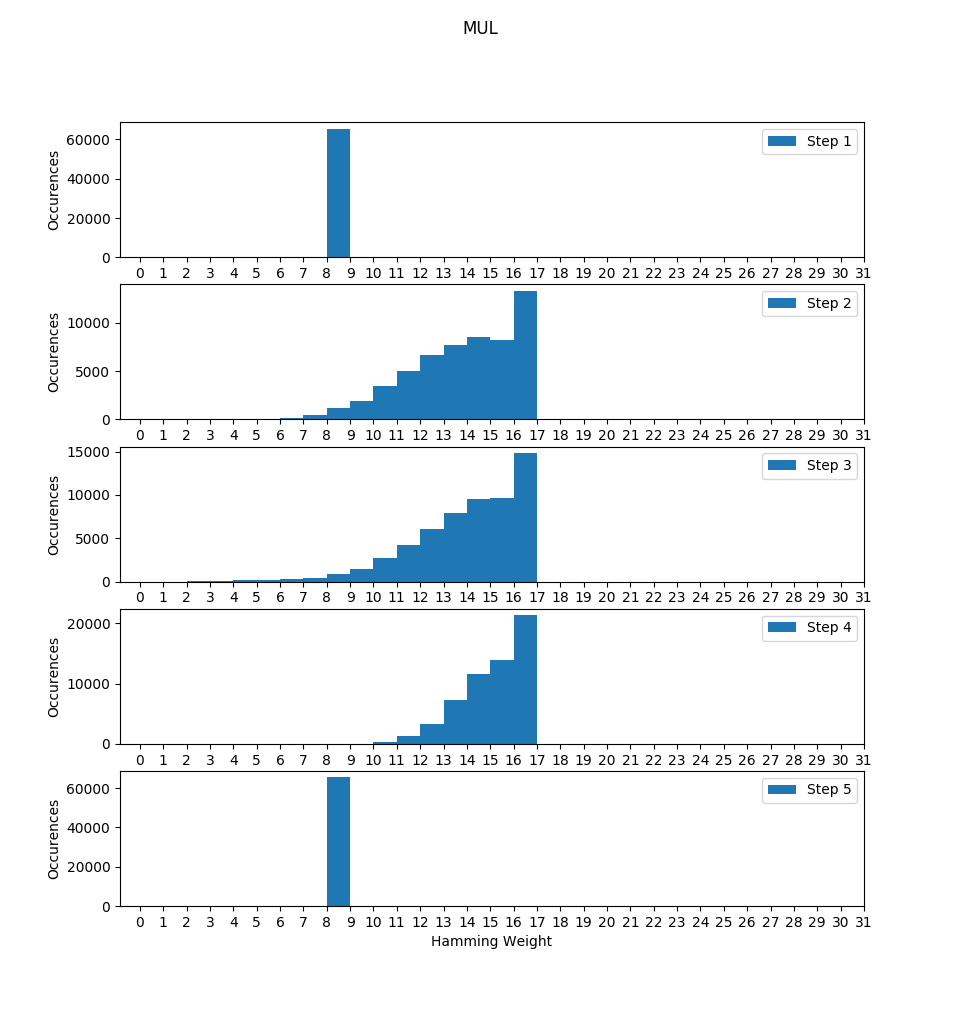
\includegraphics[width=\textwidth]{multiplication.png}
  \caption{Histogram of \hammingw s of direct balanced multiplication}
  \label{fig:mult}
\end{figure}

While \Cref{fig:mult} shows imbalanced values in the intermediate steps, it performed faster and more robust than multiplication via repeated addition.
\Cref{fig:mult-comparison} shows an evaluation of both variants, evaluated over the multiplications of all possible 8bit factors.

\begin{figure}[hp]
  \centering
  \begin{subfigure}[b]{0.49\textwidth}
    \begin{tikzpicture}
\begin{axis}[
    ybar,
    bar width=0.015\textwidth,
    enlargelimits=0.05,
    xtick={0,8,16,24,32},
    width=\textwidth
]
\addplot[pantone289,fill=pantone289!40] table [x=i, y=loop-total, col sep=comma] {data/multiplication.csv};
\end{axis}
\end{tikzpicture}

    \caption{Addition-loop multiplication}
  \end{subfigure}
  \begin{subfigure}[b]{0.49\textwidth}
    \begin{tikzpicture}
\begin{axis}[
    ybar,
    bar width=0.015\textwidth,
    enlargelimits=0.05,
    xtick={0,8,16,24,32},
    width=\textwidth,
]
\addplot[pantone289,fill=pantone289!40] table [x=i, y=direct-total, col sep=comma] {data/multiplication.csv};
\end{axis}
\end{tikzpicture}

    \caption{Direct multiplication}
  \end{subfigure}

  \begin{subfigure}[b]{\textwidth}
    \begin{tikzpicture}
\begin{axis}[
    ybar=2*\pgflinewidth,
    bar width=0.00725\textwidth,
    enlargelimits=0.05,
    xtick={0,8,16,24,32},
    width=\textwidth
]
\addplot[pantone289,fill=pantone289!40] table [x=i, y=direct-scaled, col sep=comma] {data/multiplication.csv};
\addplot[pantone144,fill=pantone144!40] table [x=i, y=loop-scaled, col sep=comma] {data/multiplication.csv};
\end{axis}
\end{tikzpicture}

    \caption{Scaled Hamming weight histograms for multiplication variants}
  \end{subfigure}
  \caption{Hamming weight histograms for direct and addition-loop multiplication}
  \label{fig:mult-comparison}
\end{figure}

